
\documentclass{article}
\usepackage{tikz}
\usepackage{pgfplots}
\usetikzlibrary{positioning}
\usetikzlibrary{fit}
\usetikzlibrary{backgrounds}
\usetikzlibrary{calc}
\usetikzlibrary{shapes}
\usetikzlibrary{mindmap}
\usetikzlibrary{decorations.text}

\begin{document}

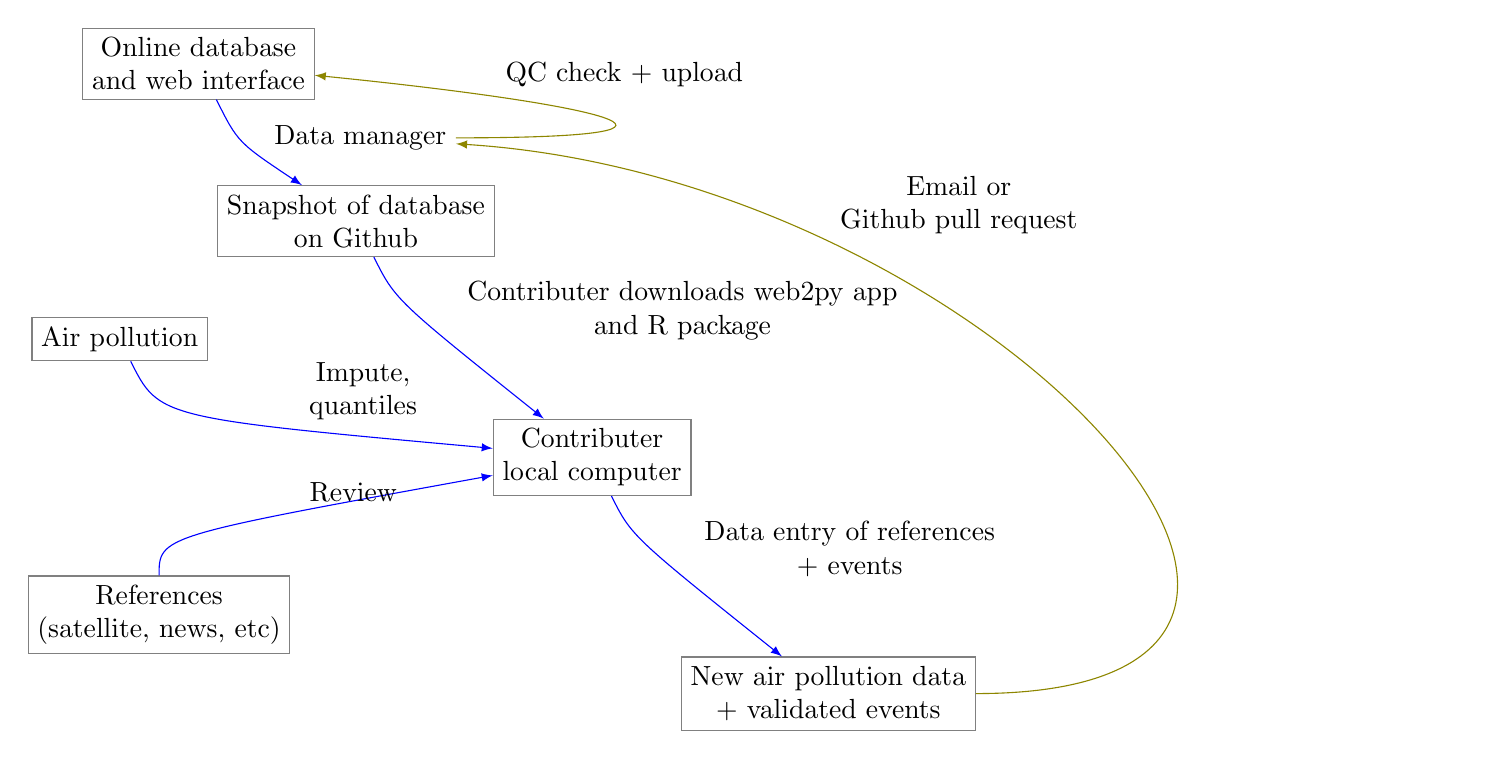
\begin{tikzpicture} [
            outpt/.style={->,blue!80!black,very thick},
            >=stealth,
         every node/.append style={align=center}]
%\tikzstyle{every node}=[draw,rectangle] 
\node (root) at (0,0) [draw=black!50,rectangle] {Online database \\ and web interface}
node (GH) at (2,-2) [draw=black!50,rectangle]{Snapshot of database \\ on Github} 
node (local) at (5,-5) [draw=black!50,rectangle]{Contributer \\ local computer}
node (AP) at (-1,-3.5) [draw=black!50,rectangle]{Air pollution}
node (ref) at (-0.5,-7) [draw=black!50,rectangle]{References \\(satellite, news, etc)}
node (validated) at (8,-8) [draw=black!50,rectangle] {New air pollution data \\ + validated events}  

 ; 
%\tikzstyle{every node}=[] 

\draw [-latex,color=blue] (root)  .. controls +(.5,-1) .. node (DM)[near end,above right,color=black, dashed] {Data manager} (GH);
\draw[-latex,color=olive] (DM) .. controls +(5,0) and +(5,-0.5) .. node[near end,above right,color=black] {QC check + upload} (root); 
\draw [-latex,color=blue] (GH) .. controls +(.5,-1) .. node (w2p)[near end,above right,color=black] {Contributer downloads web2py app\\and R package} (local);
\draw [-latex,color=blue] (AP) .. controls +(.5,-1) .. node (w2p)[near end,above right,color=black] {Impute,\\ quantiles} (local);
\draw [-latex,color=blue] (ref) .. controls +(0,1) .. node (w2p)[near end,above right,color=black] {Review} (local);
\draw [-latex,color=blue] (local) .. controls +(.5,-1) .. node (w2p)[near end,above right,color=black] {Data entry of references\\+ events} (validated);
\draw[-latex,color=olive] (validated) .. controls +(8,0) and +(8,-0.5) .. node[near end,above right,color=black] {Email or \\Github pull request} (DM); 
\end{tikzpicture} 

\end{document}
